\chapter{A Linter for Isabelle}\label{chapter:implementation} 

This chapter is the central part of the thesis: it goes through the implementation
of the linter, outlines its architecture, and showcases how it can
assist developing better Isabelle theories.
As a rolling example, we will examine the \hyperref[lint:useby]{\textit{Use by}} lint, which
suggests replacing

\begin{lstlisting}
lemma: "..."
  apply method
  apply method
  done
\end{lstlisting}
with the more compact form
\begin{lstlisting}
lemma: "..."
  by method method
\end{lstlisting}

\section{Overview and Architecture}

The linter is implemented in Isabelle/Scala. It checks the
theories based on the outer syntax (e.g. it does not process terms).
The main loop of the linter is as follows:
\begin{itemize}
    \item A document snapshot and a lint configuration 
    (\Cref{section:configuration}) are supplied to
    the linter.
    \item The document snapshot is used to extract the commands,
    which are then pre-processed to a suitable internal representation
    by saving their ranges in the source, as
    well as the ranges of each of the underlying tokens. The linter also tries to
    \textit{parse} each command into an \textit{abstract syntax tree} (AST) node.
    (\Cref{subsection:parsing}).
    \item Finally, a lint report is created (\Cref{section:reporting}) based
    on the lints specified in the configuration.
\end{itemize}
% \subsection{Interacting with the linter}
Interacting with the linter is facilitated through the 
\texttt{Linter\_Variable} class. It processes \textit{Isabelle options} to
create a suitable configuration for the linter. The variable has a binding to a
\texttt{Linter\_Interface} object which handles communication
between the linter and other Isabelle components. The interface caches the results
of linting the most recent snapshot of each document, which is a necessary 
optimization since the same report might be needed multiple times. For example, 
the Isabelle/jEdit integration of the linter underlines text in the buffer while 
displaying a detailed description of the checks in a separate panel
(see \Cref{subsection:integration-jedit} for more details).
The results' format is also customizable via the \texttt{Linter\_Variable}. 
See \Cref{section:reporting} for details on reporting.

This approach results in low coupling between the linter and any interfacing
component. For instance, the linter does not require any knowledge about
the components using it (the only dependency of the linter is Isabelle). 
From the perspective of the components using
the linter, the convenience of using the Isabelle options for configuration
eliminates the need of knowing anything about its internals. The linter consumes
the snapshots provided and the result is transformed into the desired format.
Using the \textit{variable} design, which splits invoking a component
from configuring it, is also common in the Isabelle/Scala code-base (for
example, for completion history \cite{isabelle-jedit}).
\Cref{fig:architecture-overview} shows a high-level overview of the 
interaction with the linter.

\begin{figure}[htpb]
    \centering
        \begin{tabular}{c}
\begin{tikzpicture}

    \umlsimpleclass[alias=tool, x=-3.5, y=2]{Linter\_Tool}
    \umlnote [x=-4, y=4, fill=white]{tool}{Command Line Interface}
    \umlsimpleclass[alias=PIDE, x=3.5, y=2]{jEdit}
    \umlsimpleclass[alias=variable]{Linter\_Variable}
    \umlsimpleclass[y=-2, alias=interface]{Linter\_Interface}
    \umlsimpleclass[alias=linter, y=-6]{Linter}
    \umldep[geometry=-|, mult1=Results, pos1=1.5, anchors=175 and -60]{interface}{tool}
    \umldep[geometry=|-, mult1=Snapshot, pos1=0.475, anchors=-120 and -175]{tool}{interface}
    \umldep[geometry=-|]{tool}{variable}
    \umldep[geometry=-|, arg1=Results, pos1=1.5, anchors=5 and -120]{interface}{PIDE}
    \umldep[geometry=|-, arg1=Snapshot, pos1=0.475, anchors=-60 and -5]{PIDE}{interface}
    \umldep[geometry=-|, arg1=Options, pos1=1.8]{PIDE}{variable}
    \umluniassoc{variable}{interface}
    \umldep[arg1=Snapshot,pos1=0.4, anchors=-50 and 50]{interface}{linter}
    \umldep[arg1=Configuration,pos1=0.6,anchors=-50 and 50]{interface}{linter}
    \umldep[arg1=Report, pos1=0.5, anchors=130 and -130]{linter}{interface}
    \umldep[arg1=Configuration,pos1=0.6,anchors=-50 and 50]{variable}{interface}
\end{tikzpicture}
        \end{tabular}
    \caption{Architecture Overview}\label{fig:architecture-overview}
\end{figure}
\subsection{Parsing the outer syntax}\label{subsection:parsing}
The grammar parsed by the linter is only a subset of the complete 
Isabelle grammar. This is justified for two reasons: First, most
of the grammar is not relevant for the set of lints implemented, thus
the overhead of parsing the complete grammar was spared. Second, Isabelle
theories can introduce new syntax elements at runtime that cannot be
accounted for by the developed parser. The
grammar currently recognized
represents the syntax elements related to proof methods. 
\autoref{fig:grammar} shows the railroad diagrams corresponding to that
grammar. These are from \textit{The Isabelle/Isar Reference Manual} \cite{isabelle-isar-ref}. The definition of the non-terminals 
\textit{name}, \textit{args} and \textit{nat} are omitted.

% TODO I probably need to do this locally

\begin{figure}
\noindent\makebox[\textwidth]{
\includegraphics[width=\paperwidth]{by.pdf}}
\noindent\makebox[\textwidth]{
\includegraphics[width=\paperwidth]{apply.pdf}}
\noindent\makebox[\textwidth]{
\includegraphics[width=\paperwidth]{proof.pdf}}
\noindent\makebox[\textwidth]{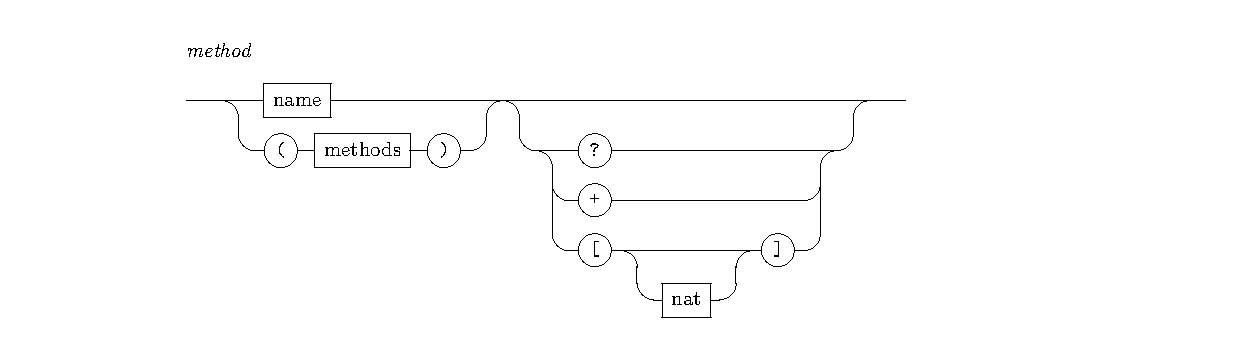
\includegraphics[width=\paperwidth]{method.pdf}}
\noindent\makebox[\textwidth]{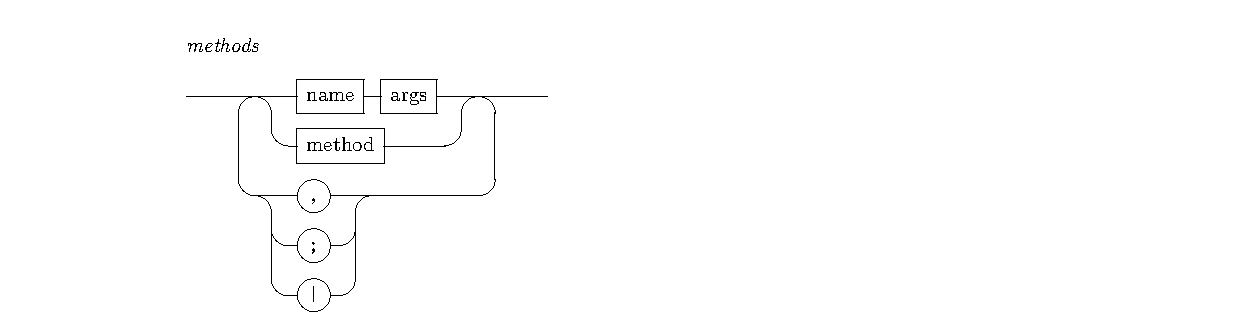
\includegraphics[width=\paperwidth]{methods.pdf}}
    \caption{Grammar parsed by the linter}\label{fig:grammar}
\end{figure}

The parsing itself is achieved through \textit{parser combinators} which is a 
well-known 
parsing technique in functional programming languages \cite{hutton1996monadic,wadler1985replace}.
The implementation builds on top of the \texttt{scala-parser-combinators}
library \cite{moors2008parser} and provides Isabelle-specific parsers.
For example, \texttt{pCommand("apply")} parses the \texttt{apply} 
token in the \texttt{apply} command, and \texttt{pMethod} parses a proof method
into its respective AST node.


\section{Lints}
\subsection{Lint abstractions}
A lint is defined by a name, a severity (either Low, Medium, or High),
and a function that takes a list of commands representing
the current document snapshot and a report; and returns a new report after
potentially adding its results.
This general abstraction is
refined further to reduce boilerplate and code duplication and 
make describing lints more convenient:
\begin{itemize}
    \item The \textit{proper commands lint} abstraction is used for
    lints that are concerned with multiple \textit{proper} commands 
    (e.g. no white-spaces or comments).
    Lints using this must provide an implementation for
    \texttt{lint\_proper}, which receives a filtered list of commands. As an
    example, the \hyperref[lint:lowlevel]{\textit{Low Level Apply Chain}} lint detects a long
    chain of single rule applications (like \texttt{simp} or 
    \texttt{rule}), which could be replaced by automated search methods.
    
    \item \textit{Single command lint} is another abstraction used
    for lints that act on one
    command. These represent the majority of the lints implemented.
    This could be used as-is, but it comes with two more refinements:
        \begin{itemize}
            \item \textit{AST Lint}, which makes use of the parsed
            AST. It allows the implementing lint to
            only focus on syntax elements that it is
            concerned with: if a lint only
            considers the \texttt{proof} commands at the start of 
            Isar-style proofs, then overriding the
            \texttt{lint\_isar\_proof} function is enough.
            An example using this abstraction is the \hyperref[lint:implicitrule]{\textit{Implicit Rule}} 
            lint, which warns about using the \texttt{rule} method without explicitly
            stating the rule used. By overriding \texttt{lint\_method},
            all that is left is to pattern-match the method supplied and
            check whether it is an implicit rule. 
            \item \textit{Parser lint}, which is useful since the parsed grammar
            does not cover all commands available in Isabelle. This offers an
            abstraction to define lints as parser combinators:
            they try to parse a lint result based on the command tokens. The 
            construction of the parsers is facilitated through the 
            Isabelle-specific parser combinators used to parse the AST.
            Next to being flexible, this approach allows for a
            declarative description of what should be avoided:
            for example, it can be used to detect when an unnamed lemma has a 
            \texttt{simp} or \texttt{cong} attribute. The
            \hyperref[lint:globalattr]{\textit{Global Attribute on Unnamed Lemma}} 
            lint implements this check.
        \end{itemize}
\end{itemize}

To avoid the boilerplate of adding the meta-data like the lint's name or 
severity, the \texttt{add\_result} method can used with \textit{proper command 
lints} and a \textit{reporter} callback with \textit{single command lints}.

The motivating example, \hyperref[lint:useby]{\textit{Use by}}, aims to express the short apply
script in a denser format. For that reason, it is a \textit{proper command lint}
with low severity. We could implemented as follows:\\
\begin{minipage}{\linewidth}
\begin{lstlisting}[language=scala]
object Use_By extends Proper_Commands_Lint {

  val name: String = "use_by"
  val severity: Severity.Level = Severity.Low
  
  def lint_proper(
    commands: List[Parsed_Command], report: Lint_Report
  ): Lint_Report = ...
\end{lstlisting}
\end{minipage}


Pattern-matching is used for finding the command sequence "lemma, apply, apply, 
done": \footnote{Other forms
can be also rewritten with "by", but they are not discussed in the 
example. The actual implementation tries to cover all cases.}
\lstset{keepspaces=true}
\begin{lstlisting}[language=scala, keepspaces=true, gobble=0]
    commands match {
      case Parsed_Command("lemma")
          :: (apply1 @ Parsed_Command("apply"))
          :: (apply2 @ Parsed_Command("apply"))
          :: (done @ Parsed_Command("done"))
          :: next => ... // Update the report, 
                          // continue checking the remaining commands
      case ... // The rest of the cases
    }
\end{lstlisting}
Thereupon, all that is left is to generate the replacement and update the
report, which we continue in \autoref{section:reporting}.

\subsection{The Lint Store}
The \texttt{Lint\_Store} is like a repository that allows referencing lints by 
their
names. Lints can be registered at runtime, which is useful when the linter is used as 
a library or Scala code is run interactively in Isabelle theories.
This permits externally defined checks to be integrated seamlessly with the linter.

Adding to that, the store introduces the concept of \textit{bundles}.
Bundles are groups of lints that can be used together. Depending on
the context, the set of lints used can be different: it might be acceptable
to have interactive commands like \texttt{sledgehammer} while
developing proofs in Isabelle/jEdit, but not when trying to submit an entry
to the AFP. Bundles can be presets intended to be used
on their own (like a preset for interactive proof development) or
to group lints that are related (like a bundle to prohibit
interactive commands). As is the case with lints, bundles can also be
registered at runtime.

\section{Lint Reporting}\label{section:reporting}

When a lint is triggered, it creates a \texttt{Lint\_Result} 
containing all the relevant information: the name of the lint and its
severity, a message briefly explaining the lint, the range in the
document that is problematic, the list of commands related to the
lint as well as an optional \texttt{Edit} that specifies a range in the
document and with what it should be replaced. These results are accumulated in a 
\texttt{Lint\_Report}, which is basically a wrapper around a list 
of results with some convenience
methods, like getting the results for a specific command.

Back to our \texttt{use\_by} example. To generate the replacement for
\begin{lstlisting}
apply method1
apply method2
done
\end{lstlisting}
we can use parser combinators to extract the method: parse and ignore the
\texttt{apply} token followed by a potential white-space, and return the rest of
the tokens as a string:
\begin{lstlisting}[language=scala]
  private def removeApply: Parser[String] = (
    (pCommand("apply") ~ pSpace.?) // Parse apply, followed by a 
potential white space
      ~> // Ignore what is already parsed
        pAny.* // Accept everything that follows..
        ^^ mkString // .. and turn it to a string
  )
    
  private def gen_replacement(
    apply_script: List[Parsed_Command]
  ): Option[String] =
    apply_script match {
      case apply1 :: apply2 :: done :: Nil =>
        for {
          method1 <- tryTransform(removeApply, apply1)
          method2 <- tryTransform(removeApply, apply2)
        } yield s"by $method1 $method2"
      case  ... // omitted
    }

\end{lstlisting}
All that is left is to add the result to the current report using the 
\texttt{add\_result} method:
\begin{lstlisting}[language=scala]
  private def report_lint(
    apply_script: List[Parsed_Command], report: Lint_Report
  ): Lint_Report = {
    val new_report = for {
      replacement <- gen_replacement(apply_script)
    } yield add_result(
      """Use "by" instead of a short apply-script.""",
      list_range(apply_script.map(_.range)),
      Some(Edit(list_range(apply_script map (_.range)), replacement)),
      apply_script,
      report
    )
    new_report.getOrElse(report)
  }
  
\end{lstlisting}

The described \texttt{Lint\_Result} and \texttt{Lint\_Report} structures
are intended to be used \textit{internally} by 
the linter. Through Reporters, the reports can be transformed into a suitable format
depending on the context. Three reporters are implemented for these purposes:

\begin{itemize}
    \item \texttt{XML\_Lint\_Reporter}: returns an \texttt{XML}
    representation of the report.
    \item \texttt{JSON\_Reporter}: returns a \texttt{JSON} 
    representation of the report.
    \item \texttt{Text\_Reporter}: returns a textual representation
    of the report.
\end{itemize}

These reporters are all currently in use: \texttt{XML} is useful
within Isabelle as with the Isabelle/jEdit integration;
\texttt{JSON} and text are used with the command line interface of the
linter (see \autoref{section:integration} for more details).

\section{Lint Configuration}\label{section:configuration}
Users should have full control over exactly what lints they want to 
enable. This is crucial, as the context highly influences which checks
are relevant: for example, using the \texttt{axiomatization} command
is necessary to create a new logic, but it might result in 
inconsistencies if carelessly used in formalizations. Configurability
is achieved through
the \texttt{Linter\_Configuration} class. It can be used to enable or
disable individual lints, as well as bundles. The selection
is based on names, which are subsequently used to fetch the corresponding 
lints with the help of the \texttt{Lint\_Store}.
\subsection{Options}\label{subsection:options}
Isabelle manages persistent settings through \textit{options}. These
are stored under \texttt{\$ISABELLE\allowbreak 
\_HOME\_USER/etc/preferences} and managed through Isabelle/Scala. The
linter defines a set of configuration options that get applied when
interacting with the linter through the \texttt{Linter\_Variable}:
\begin{itemize}
    \item \texttt{linter} specifies whether the linter is enabled.
    \item \texttt{enabled\_bundles} is comma-separated list of the names
    of the bundles to be enabled.
    \item \texttt{enabled\_lints} and \texttt{disabled\_lints} are
    additionally two comma-separated lists of the names of lints to be
    enabled or disabled, respectively.
\end{itemize}
The last three options are used to generate a corresponding
\texttt{Lint\_Configuration}, by first adding the specified bundles
and enabled lints and then removing the disabled lints.

\section{Integration}\label{section:integration}
\subsection{Isabelle/jEdit Integration}\label{subsection:integration-jedit}
Isabelle/jEdit is the default user-interface and IDE when working with
Isabelle, so it was important to integrate the linter with it.
The coupling is realized through the PIDE plugin, by providing a
binding to a \texttt{Linter\_Variable} with a \texttt{XML\_Reporter}. 
The developed integration provides both feedback on the lints
discovered in the active theory, as well as configuration options to
customize the behavior of the linter.

\subsubsection{Feedback}
The results of linting the current theory are available 
through three main sources (as shown in \autoref{fig:jedit-buffer}):
\begin{itemize}
    \item \textit{Underlined text} in the main buffer with
    a color based on the severity of the lint.
    \item \textit{The output panel} (at the bottom)
    is central to the interaction with Isabelle/jEdit since it shows 
    the prover messages of the command under the caret. 
    The lints for that command are also appended to the output panel.
    The displayed 
    lints are sorted in descending order of severity.
    \item \textit{The linter panel} (at the right) 
    is a new panel introduced specifically for the linter. Like
    the output panel, it displays lints regarding the
    current command. Furthermore, it provides a more general
    overview of the entire theory, with each lint's severity, name, and
    location included.
\end{itemize}

\begin{figure}[htpb]
    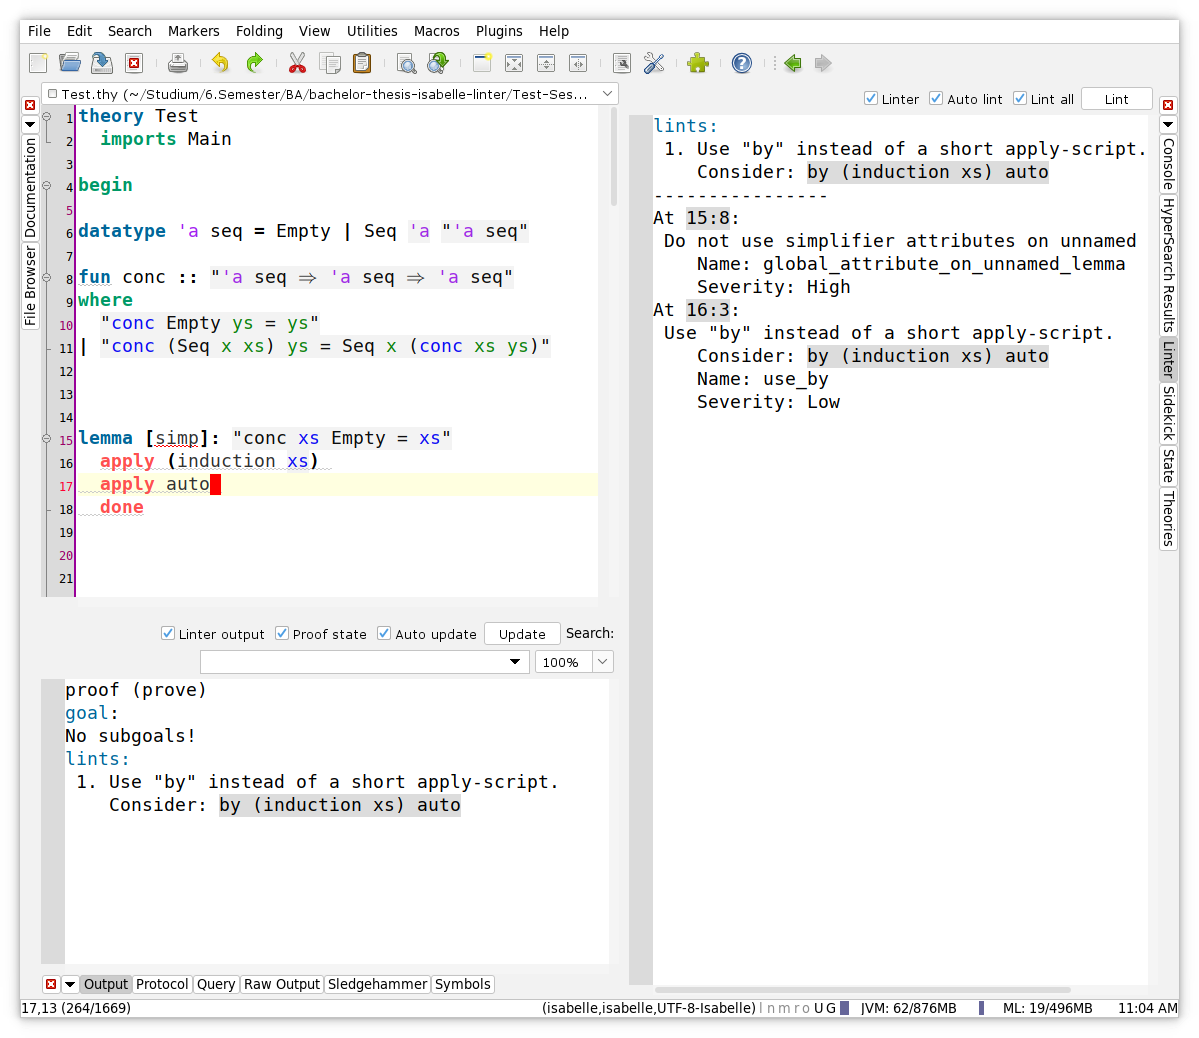
\includegraphics[width=\textwidth]{images/jedit-buffer.png}
    \caption{Isabelle/jEdit with linter integration}\label{fig:jedit-buffer}
\end{figure}

Both panels make it possible to automatically apply lint 
suggestions. The suggestions are displayed in the panels with a grey
background (see \autoref{fig:jedit-buffer}). The linter panel also
enables navigation to the lint location, by clicking on the reported lint
positions (also with a grey background).

To achieve this interactivity, the linter defines two special markups
(\textit{lint\_edit} and \textit{lint\_position}) and adds them
to the list of active markups in Isabelle/jEdit. When the user clicks
on text marked with these markups, jEdit goes through the defined handlers 
\footnote{defined in \texttt{src/Tools/jEdit/src/services.xml}} which
perform the actions needed based on the type of markup. 

Isabelle users might recognize this feature from using \texttt{sledgehammer}:
the found proofs are displayed with a grey background, and upon
clicking on them, they get inserted into the buffer. This is implemented
in the same way as the linter feature: \texttt{sledgehammer} wraps
the proofs in the \textit{sendback} active markup, and the default
active markup handler of Isabelle/jEdit handles inserting the proof.

\subsubsection{Configuration options}
Adding to the options in \autoref{subsection:options}, five additional
ones are used exclusively for Isabelle/jEdit:
\begin{itemize}
    \item \texttt{lint\_all} indicates whether the lints of the
    whole document should be included in the linter panel
    \item \texttt{lint\_output\_panel} indicates whether the lints are
    added to the output panel
    \item \texttt{linter\_high\_color}, \texttt{linter\_medium\_color} 
    and \texttt{linter\_low\_color} indicate the color of the
    underline.
\end{itemize}

The first two options and the ones described in
\autoref{subsection:options} are available to view and edit  under 
\textit{Plugins / Plugin Options / Isabelle / General / Linter} (together
with the rest of the Isabelle options). The color-specific options can be
customized under \textit{Plugins / Plugin Options / Isabelle / 
Rendering}.

The output panel comes with an additional checkbox to control whether
the linter output is appended to the prover output. The linter panel
has controls to toggle the linter plugin entirely, to indicate whether
its output should be updated automatically, to control whether the
lints of the whole document should be displayed, and a button to trigger
a lint (useful when auto-linting is disabled). These are displayed in
\autoref{fig:jedit-buffer}.

\subsubsection{Updating results}

The linter Isabelle/jEdit integration is implemented in an 
event-driven approach. A subclass of \textit{Linter\_Variable}, called
\textit{PIDE\_Linter\_Variable}, listens to changes in the commands
or the global options. When such event is dispatched, it lints
the current snapshot in parallel
and notifies the listening components
when it is done \footnote{This is achieved by emitting a 
\textit{Caret Focus} event. Ideally, a separate event for the linter
should be added, but that requires more changes to the PIDE plugin. This
can be added when a tighter linter integration is required.}
so they can react accordingly.

\subsection{The \texttt{isabelle lint} Command Line Tool}
With the \texttt{isabelle lint} tool the linter can be run from the
command line. It has the following usage:
\begin{lstlisting}[keepspaces=true]
Usage: isabelle lint [OPTIONS] SESSION

  Options are:
    -b NAME      base logic image (default "Pure")
    -d DIR       include session directory
    -o OPTION    override Isabelle system OPTION (via NAME=VAL or NAME)
    -v           verbose
    -V           verbose (General)
    -r MODE      how to report results (either "text", "json" or "xml",
    default "text")
    -l           list the enabled lints (does not run the linter)

  Lint isabelle theories.

\end{lstlisting}
The options are as follows:
\begin{itemize}
\item Option \texttt{-b} provides a base logic image, as used in
          \texttt{isabelle dump} \cite{isabelle-system}.
          
\item Option \texttt{-d} allows adding more directories to have access
to more sessions.

\item Option \texttt{-v} increases the verbosity level of the linter.

\item Option \texttt{-V} increases the general verbosity level.

\item Option \texttt{-o} enables overriding Isabelle options. This can be
primarily used to configure the linter by overriding the relevant
options: \texttt{enabled\_bundles}, \texttt{enabled\_lints} and
\texttt{disabled\_lints}. The \texttt{linter} option is ignored: it does not
matter what value it has, the linter will be enabled regardless.

\item Option \texttt{-l} generates a lint configuration based on the Isabelle
options, and prints the results. If this option is set, the linter does
not run.

\item Option \texttt{-r} specifies the reporting mode, which can be 
\texttt{text}, \texttt{xml}, or \texttt{json}. The \texttt{text} mode provides
results in a human-readable format. \autoref{fig:lint-text-example} shows
an example of its usage. On the other hand, both \texttt{json} and
\texttt{xml} options
can be used to provide a machine-readable output, which is convenient because
the results can be processed further, for example to create warnings as a part
of a CI/CD pipeline or to analyze the findings (as done in \autoref{chapter:evaluation}). Example outputs of these two modes can be found
int \autoref{app:xml-json}.
\begin{figure}
   \begin{lstlisting}
$ isabelle lint -v HOL
Loading 2 sessions ...
Starting session Pure ...
Loading 111 theories ...
...
Processing theory HOL.Inductive ...
At 203:3:                [use_by]
  Use "by" instead of a short apply-script.
  Severity: LOW

apply (erule gfp_upperbound [THEN subsetD])
  apply (erule imageI)
  done

  Suggestion: by (erule gfp_upperbound [THEN subsetD]) (erule imageI)
 ...
    \end{lstlisting}
    \caption{Output of 
    \texttt{isabelle lint} text mode}\label{fig:lint-text-example}
\end{figure}


\end{itemize}


The tool invokes the linter through a
\texttt{Linter\_Variable}, as is the case with the Isabelle/jEdit
integration, in order to handle Isabelle options. The main difference
between the two interfaces is that the tool does not cache lint results
since they are only needed once.
The tool works similarly to the 
\texttt{isabelle dump} command; by 
processing the PIDE session database on the spot \cite{isabelle-system}.
This is the cause behind the main limitation of \texttt{isabelle lint}:
it is slow (see \Cref{chapter:evaluation}). The bottleneck is not the linting 
but it is rather generating the snapshot. The provided session and all its dependencies
need to be processed. Processing \texttt{HOL} alone requires substantial
memory and time \cite{isabelle-system}. Option \texttt{-b} 
allows overcoming this problem by providing a base logic image which will be
skipped. A possible faster alternative is to rely on the build database
to access the document snapshots instead of generating them
directly. However, \textit{Isabelle2021} does not provide access to 
the command spans through the build database, which makes the snapshot
unusable for the linter: the whole theory is one unparsed command.